\documentclass[12pt]{article}

\usepackage{graphicx,amsmath}
\usepackage[margin=1in]{geometry}
\usepackage{float}

\title{CMDA 3634 PSA02 : OpenMP $k$-means on ARC}
\author{Jason Bruno Terceros}
\date{\today}

\begin{document}

\maketitle

In this write-up we consider running our OpenMP $k$-means on ARC. We will also be implementing our code by making it parallel and using static scheduling. This will be done by adjusting two functions in code that is provided to us. Finally, we will run our code and produce images out to visually see how our code produced these images on ARC.

\textbf{OpenMP $k$-means}

In a previous assignment you implemented Lloyd’s algorithm with initial cluster centroids chosen using the farthest first algorithm to approximate a solution to the k-means clustering problem. In this assignment, you are given a full sequential source code in the file \text{omp\_kmeans.c}. You will modify the included source code to implement a parallel version using OpenMP of both the farthest first algorithm to choose the initial cluster centers and Lloyd’s algorithm for approximating a solution to the k-means problem. You will test, demonstrate, and analyze the parallel performance of each algorithm separately on ARC. For this assignment we will only be working with the MNIST test set with 10000 handwritten digit images.


\section{OpenMP Farthest First Implementation Tasks}

\begin{enumerate}
    \item Coding Tasks

We pulled the latest updates from our cmda3634\_materials repo in ARC
\begin{verbatim}
git add *.c
git commit -m "starter source file for PSA02"
git push
\end{verbatim}

We were told to modify our function calc\_arg\_max in our file omp\_kmeans.c. We needed to implement this code to the part of the farthest first algorithm that calculates the arg max in parllel using OpenMP.

\textbf{Modified code:}
\begin{verbatim}
int calc_arg_max (double data[], int num_points, 
                    int dim, int centers[], int m) 
{
    int arg_max;
    double cost_sq = 0;

#pragma omp parallel default(none) shared(arg_max, cost_sq, 
                        dim, data, num_points, centers, m)
{
    int thread_arg_max;
    double thread_cost_sq = 0;

    #ifdef DYNAMIC
    #pragma omp for schedule(dynamic)
    #else
    #pragma omp for schedule(static)
    #endif

    for (int i=0;i<num_points;i++) 
    {
        double min_dist_sq = DBL_MAX;
        for (int j=0;j<m;j++) 
        {
            double dist_sq = vec_dist_sq
                        (data+i*dim,data+centers[j]*dim,dim);
            if (dist_sq < min_dist_sq) 
            {
                min_dist_sq = dist_sq;
            }
        }

        if (min_dist_sq > thread_cost_sq) 
        {
            thread_cost_sq = min_dist_sq;
            thread_arg_max = i;
        }
    }
    #pragma omp critical
    {
        if (thread_cost_sq > cost_sq) 
        {
            cost_sq = thread_cost_sq;
            arg_max = thread_arg_max;
        }
    }
}
    return arg_max;
}
\end{verbatim}

    \item Testing Tasks
Now we will test our farthest first implementation in isolation we will run $k$-means with m=0.
Run the script omp\_farfirst.sh using sbatch to test your parallel farthest first implementation.
\begin{verbatim}
sbatch omp_kmeans.sh mnist_test.dat 25 0
\end{verbatim}

then we ran our OpenMP kmeans code using k=25 and m=0. Next type
\begin{verbatim}
module load matplotlib
cat omp_kmeans.out | python3 mnist25.py mnist_test_25_0.png
\end{verbatim}

We should generate an image of the 25 MNIST centers.
Figure  
\ref{mnist_test_25_0.fig} 
shows our image of the 25 MNIST centers. We compared Figure \ref{mnist_test_25_0.fig} and found that it is similar to our provided example.

\begin{figure}[H]
\begin{center}
    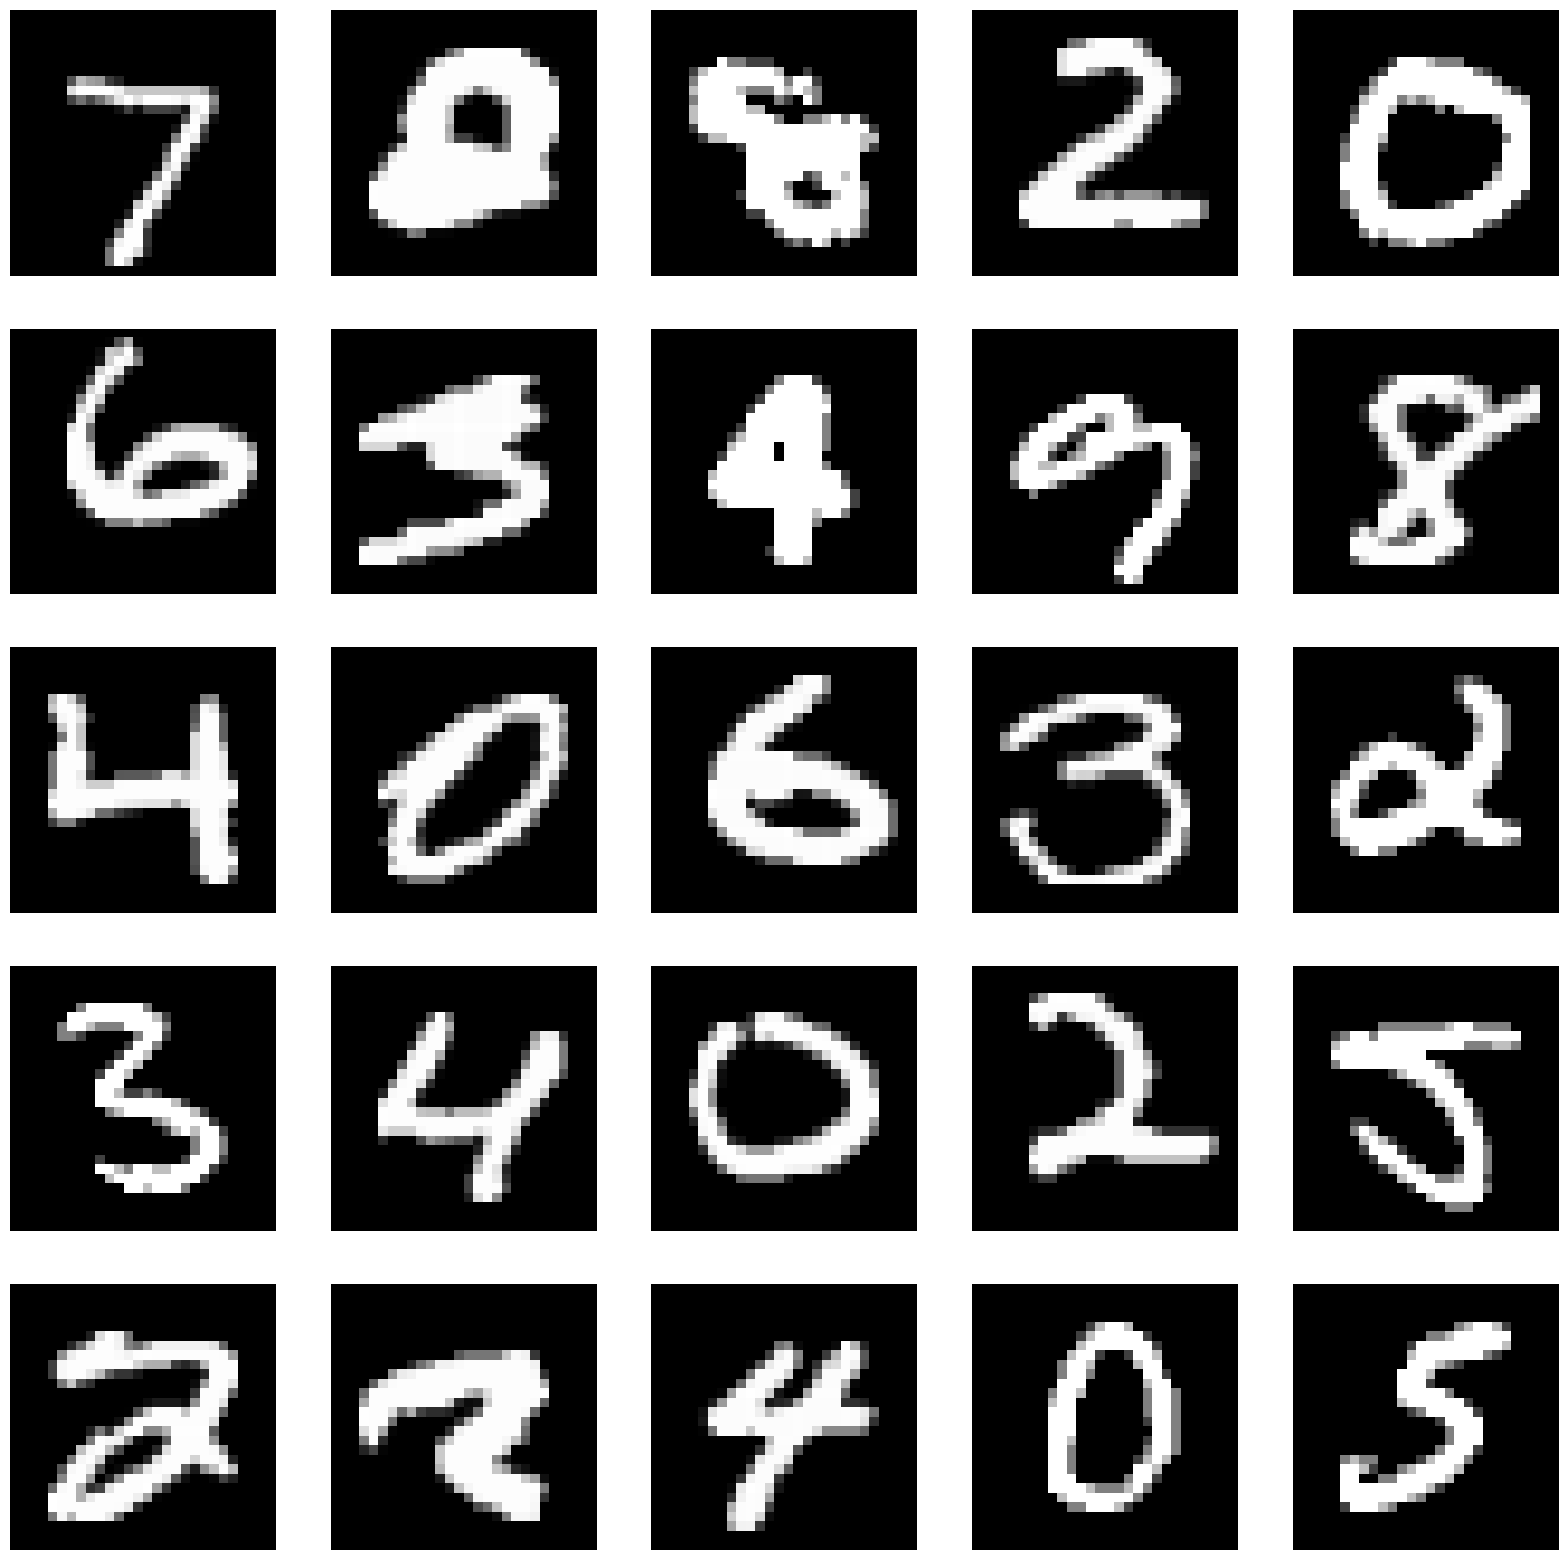
\includegraphics[width=0.65\textwidth]{images/mnist_test_25_0.png}
\end{center}
\caption{mnist Image of k=25 and m=0}
\label{mnist_test_25_0.fig}
\end{figure}


We also went on to test the parallel performance of my code by typing:
\begin{verbatim}
sbatch omp_kmeans_timing.sh mnist_test.dat 25 0
\end{verbatim}

Figure  
\ref{kmeans_timing_25_0.fig} 
shows our output for a parallel performance when k=25.

\begin{figure}[H]
\begin{center}
    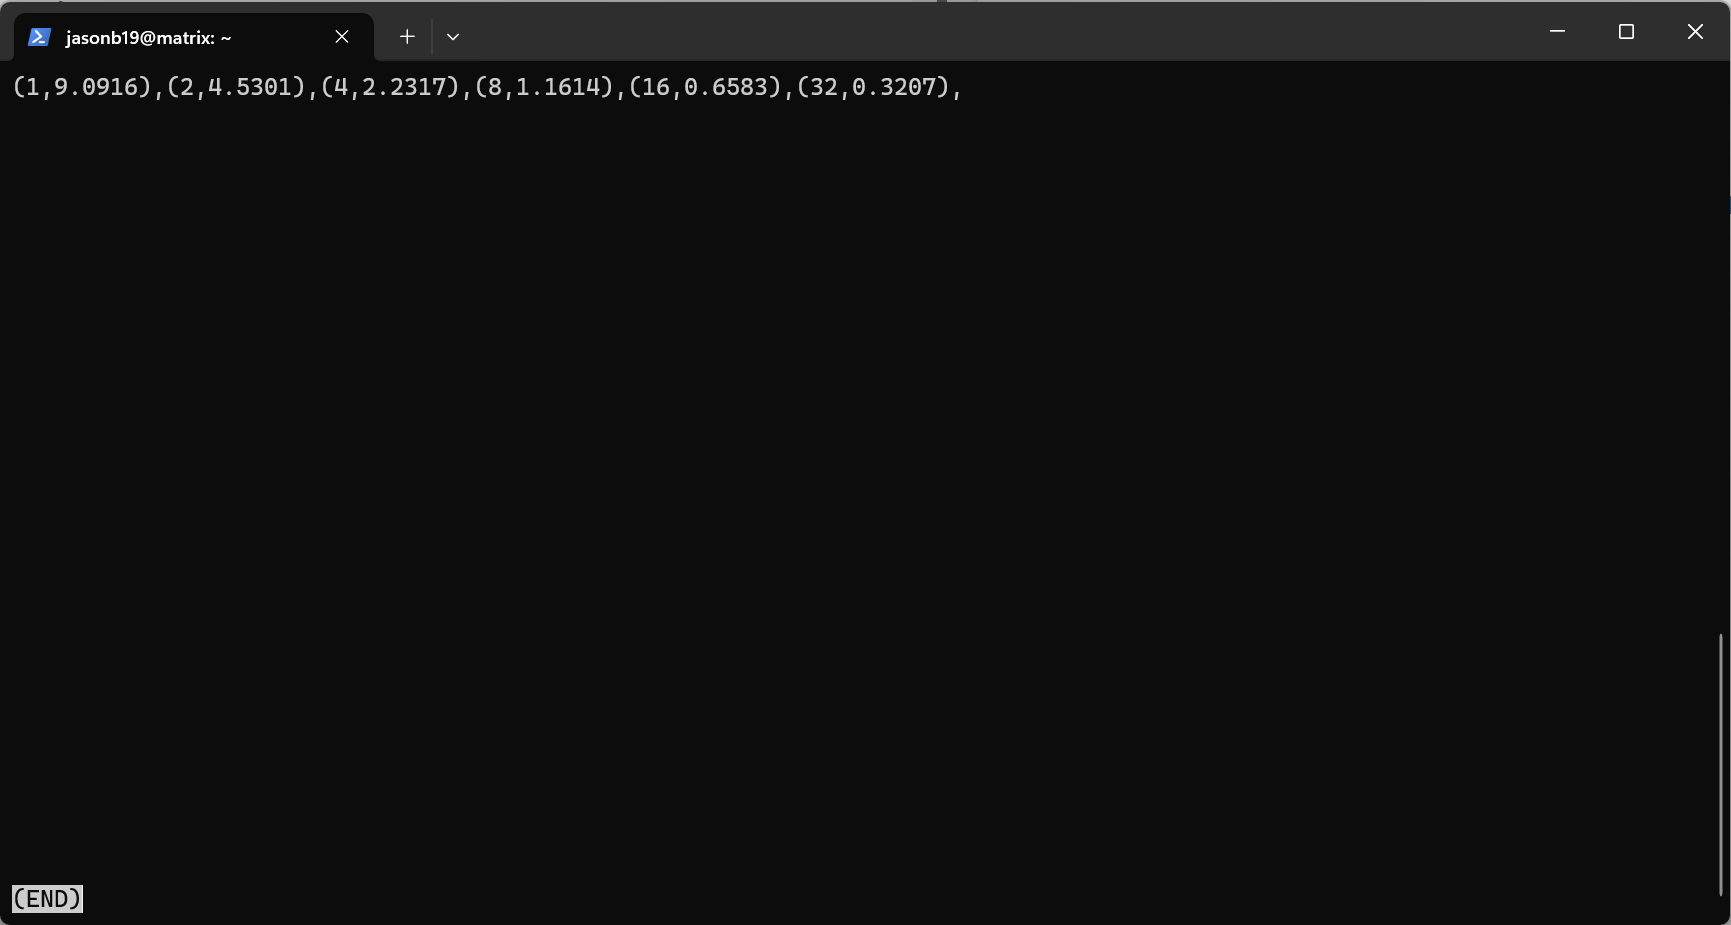
\includegraphics[width=0.95\textwidth]{images/kmeans_timing_25_0.png}
\end{center}
\caption{Parallel Performance for k=25 and m=0}
\label{kmeans_timing_25_0.fig}
\end{figure}

The corresponding strong scaling study of my output is produced:
\begin{verbatim}
[jasonb19@tinkercliffs2 PSA02]$ more omp_kmeans_timing.out
(1,9.0916),(2,4.5301),(4,2.2317),(8,1.1614),(16,0.6583),(32,0.3207),
\end{verbatim}

Figure  
\ref{plot_25_0.fig} 
is my produced plot for a strong scaling study.

\begin{figure}[H]
\begin{center}
    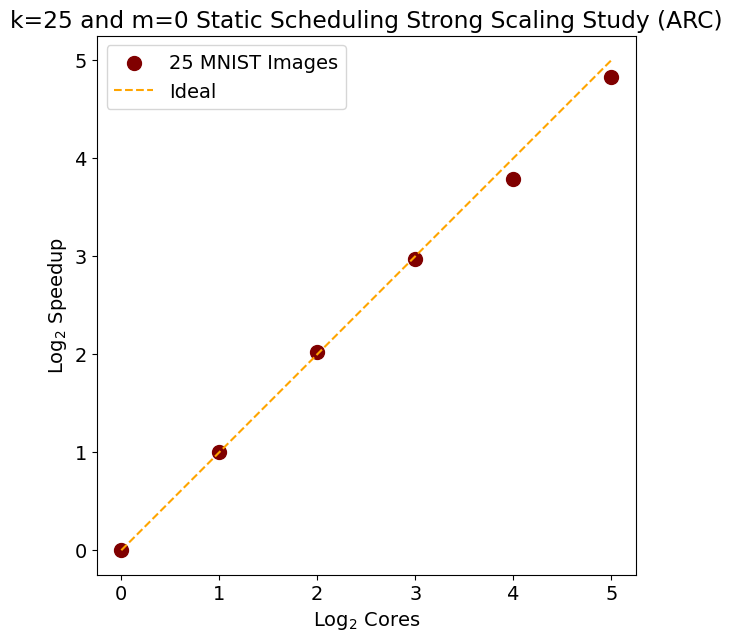
\includegraphics[width=0.95\textwidth]{images/plot_25_0.png}
\end{center}
\caption{Strong Scaling Study for k=25 and m=0 OpenMP}
\label{plot_25_0.fig}
\end{figure}


\end{enumerate}

% end of section 1

\section{OpenMP $k$-means Implementation Tasks}


\begin{enumerate}
    \item Coding Tasks
We were told to modify our function calc\_kmeans\_next in our file omp\_kmeans.c. We need to implement the part of Lloyd's algorithm that updates the $k$ means in parallel using OpenMP. I was also informed to use the functions provided in vec.c to improve my codes' readability.

\textbf{Modified code:}
\begin{verbatim}
void calc_kmeans_next (double data[], int num_points, 
            int dim, double kmeans[], double kmeans_next[], int k) 
{
    int cluster_size[k];
    for (int i=0;i<k;i++) 
    {
        cluster_size[i] = 0;
    }
    vec_zero(kmeans_next,k*dim);

#pragma omp parallel default(none) 
    shared(cluster_size, k, dim, num_points, kmeans, data, kmeans_next)
{
    int thread_cluster_size[k];
    for (int i=0;i<k;i++) 
    {
        thread_cluster_size[i] = 0;
    }
    double thread_kmeans_next[k*dim];
    vec_zero(thread_kmeans_next,k*dim);

    #ifdef DYNAMIC
    #pragma omp for schedule(dynamic)
    #else
    #pragma omp for schedule(static)
    #endif
    for (int i=0;i<num_points;i++) 
    {
        int cluster = find_cluster(kmeans,data+i*dim,k,dim);
        double* kmean = thread_kmeans_next+cluster*dim;
        vec_add(kmean,data+i*dim,kmean,dim);
        thread_cluster_size[cluster] += 1;
    }

    #pragma omp critical
    {
        for (int i = 0; i < k; i++)
        {
            cluster_size[i] += thread_cluster_size[i];
        }
        vec_add(kmeans_next,thread_kmeans_next,kmeans_next,k*dim);
    }
}
    for (int i=0;i<k;i++) 
    {
        double* kmean = kmeans_next+i*dim;	
        if (cluster_size[i] > 0) 
        {
            vec_scalar_mult(kmean,1.0/cluster_size[i],kmean,dim);
        } else {
            printf ("error : cluster has no points!\n");
            exit(1);
        }
    }
}
\end{verbatim}

    \item Testing Tasks
We will run our script omp\_farfirst.sh using sbatch to test my parllel farthest first implementation.
\begin{verbatim}
sbatch omp_kmeans.sh mnist_test.dat 16 40
\end{verbatim}
We will run the OpenMP kmeans code using k=16 and m=40. We typed:
\begin{verbatim}
cat omp_kmeans.out | python3 mnist16.py mnist_test_16_40.png
\end{verbatim}
This will give us an image of the 16 MNIST cluster centers.
Figure  
\ref{mnist_test_16_40.fig} 
shows our image of the 16 MNIST centers. We compared Figure \ref{mnist_test_16_40.fig} and found that it is similar to our provided example.

\begin{figure}[H]
\begin{center}
    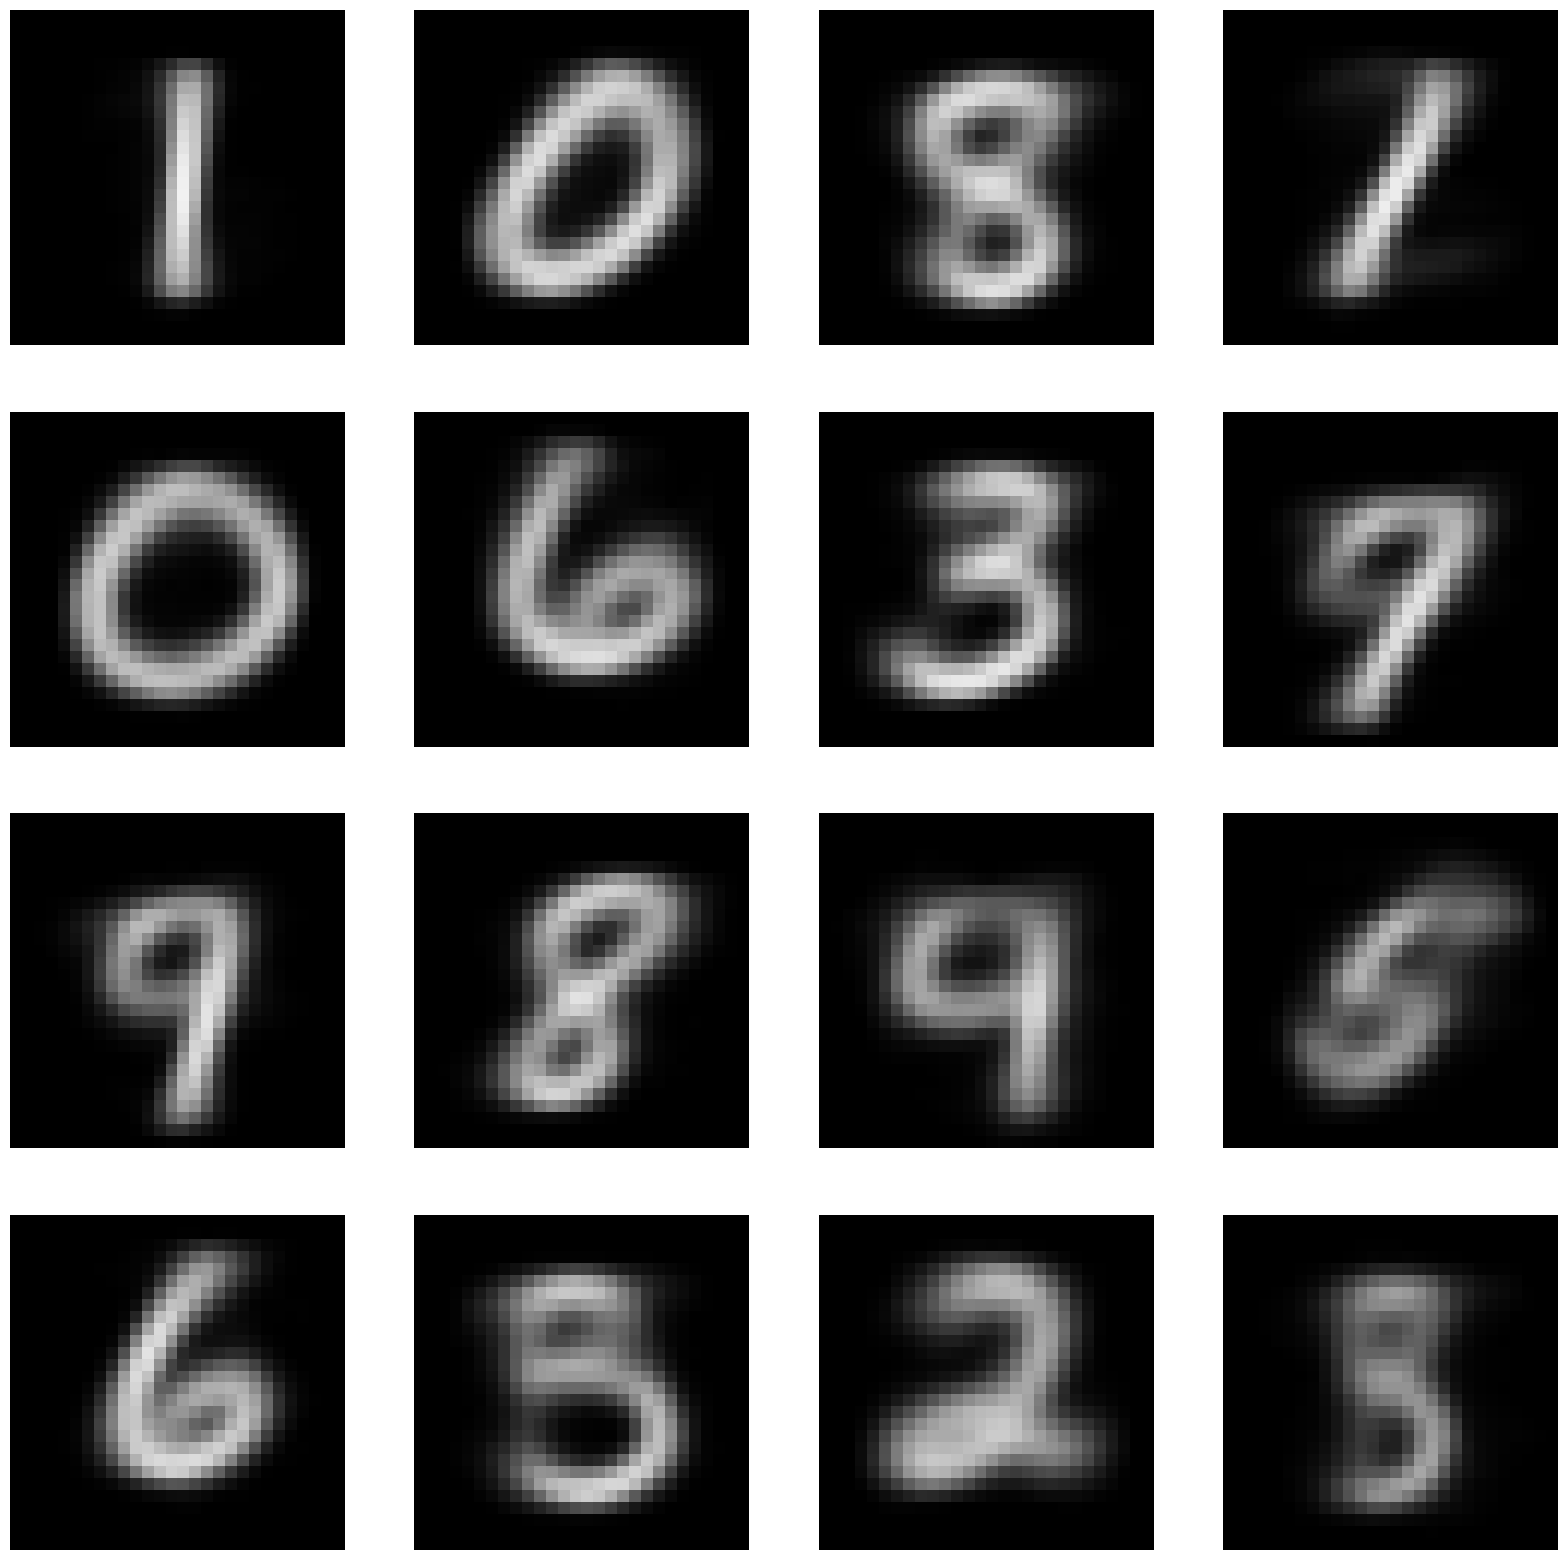
\includegraphics[width=0.65\textwidth]{images/mnist_test_16_40.png}
\end{center}
\caption{mnist Image of k=16 and m=40}
\label{mnist_test_16_40.fig}
\end{figure}

Next, we tested the parallel performance of my code. We rab my OpenMP fast farfirst code using k=16 and m=40 with different thread counts. We ran this to get my strong scaling study values:

Figure  
\ref{kmeans_timing_16_40.fig} 
shows our output for a parallel performance when k=16.

\begin{figure}[H]
\begin{center}
    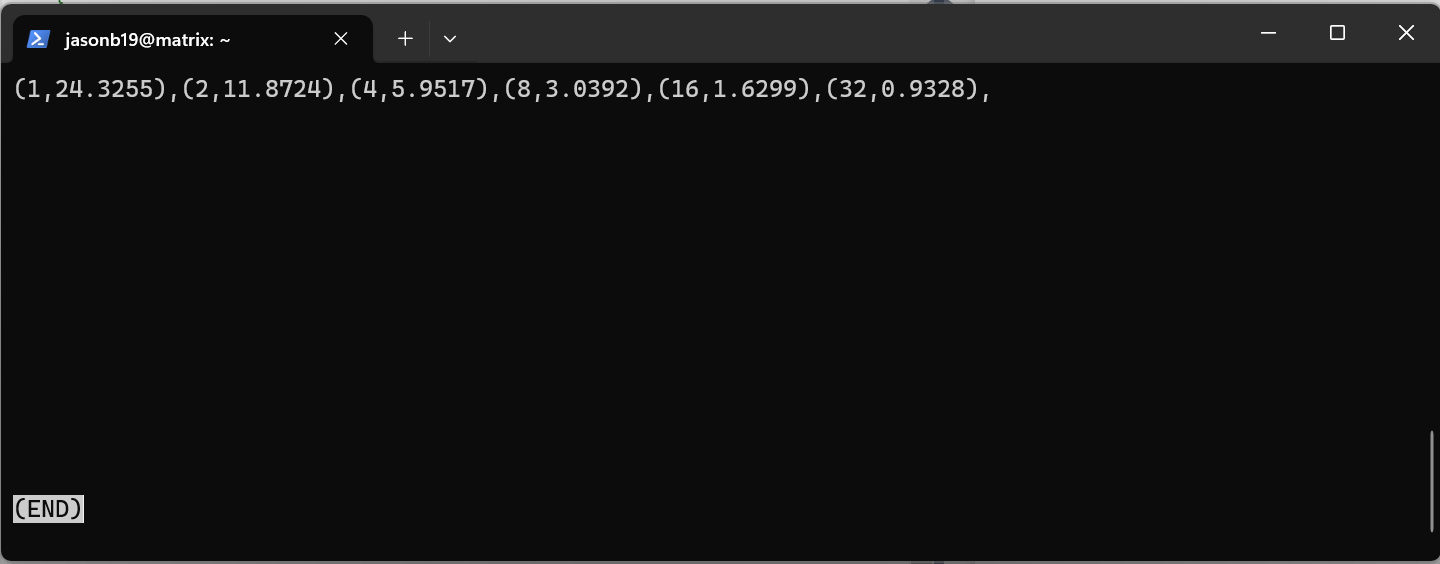
\includegraphics[width=0.95\textwidth]{images/kmeans_timing_16_40.png}
\end{center}
\caption{Parallel Performance for k=16 and m=40}
\label{kmeans_timing_16_40.fig}
\end{figure}
    
\end{enumerate}

The corresponding strong scaling study of my output is:
\begin{verbatim}
[jasonb19@tinkercliffs2 PSA02]$ more omp_kmeans_timing.out
(1,24.3255),(2,11.8724),(4,5.9517),(8,3.0392),(16,1.6299),(32,0.9328),
\end{verbatim}


Figure  
\ref{plot_16_40.fig} 
is my produced plot for a strong scaling study.

\begin{figure}[H]
\begin{center}
    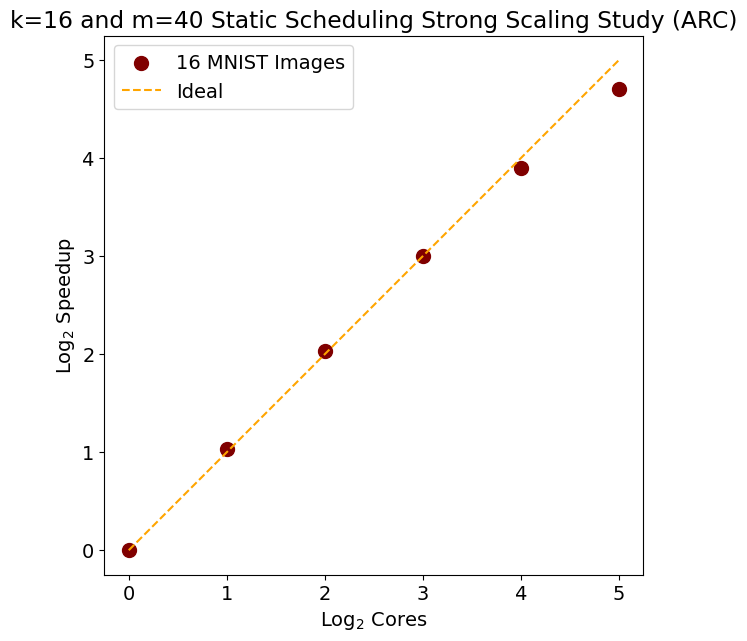
\includegraphics[width=0.95\textwidth]{images/plot_16_40.png}
\end{center}
\caption{Strong Scaling Study for k=16 and m=40 OpenMP}
\label{plot_16_40.fig}
\end{figure}

% end of section 2

\section{Farthest First Conceptual and Demonstration Tasks}

\begin{enumerate}
    \item Classification of Each Variable
% arg_max, cost_sq, dim, data, num_points, centers, m
When evaluating my parallel code, I would review my entire code to see where I can reference my shared variables and private ones. Further examining my code I found that there is only one write variable used, arg\_max. It is used in my omp critical at the very end. We have plenty of read only variables and only one that is both read-write. cost\_sq is the only read-write variable. It is used in the if-statement condition checking if our private variable thread\_cost\_sq is greater than cost\_sq and then if it is, setting that thread\_cost\_sq to my new cost\_sq. Hence, I am reading it in my conditional statement and then changing it when it fits my condition. Finally, I do believe the remainder of my shared variables are all read only, that being; dim, data, num\_points, centers, m.

    \item Steps Took to Make Code Run Efficiently in Parallel

I began by creating new variables for my parallel region that will follow my arg\_max and my cost\_sq respectively, thread\_arg\_max and thread\_cost\_sq. This is because while in parallel they have been checked and or changed throughout. This is mainly towards the end of my parallel region when we begin to check if min\_dist\_sq is greater than cost\_sq, except now we change it to thread\_cost\_sq since we will check cost\_sq once at the end in our omp critical. The same is true for arg\_max. This allows to code to run as it would be excepted when having to read values, and only changing at the end when necessary. Read our variables won't have an effect on our final output until we are fully done running through our parallel.

    \item Explanation of Determining Type of Scheduling

For the farthest first algorithm, I incorporated our IF-ELSE condition for if we run DYNAMIC or for our code to run static when prompted. This section comes right before our for-loop and right after instantiating our private thread variables. code:
\begin{verbatim}
 #ifdef DYNAMIC
#pragma omp for schedule(dynamic)
#else
#pragma omp for schedule(static)
#endif
\end{verbatim}
As such, we officially ran our code as static since in compilation I do not believe we called DYNAMIC. I believe we ran static scheduling because our code needed to run in a sequence to find the maximum distance and the minimum cost of the data. I would have to evaluate the one point with another, and then move one to do the same with the next and so one effectively needing to be ordered in a certain way.

    \item Farthest First Test Task 2 with k = 36 and m = 0

We will repeat the farthest first testing task with the new provided values for k and m. Hence, this will be 36 and 0 respectively.
Figure  
\ref{mnist_test_36_0.fig} 
shows our image of the 25 MNIST centers. 

\begin{figure}[H]
\begin{center}
    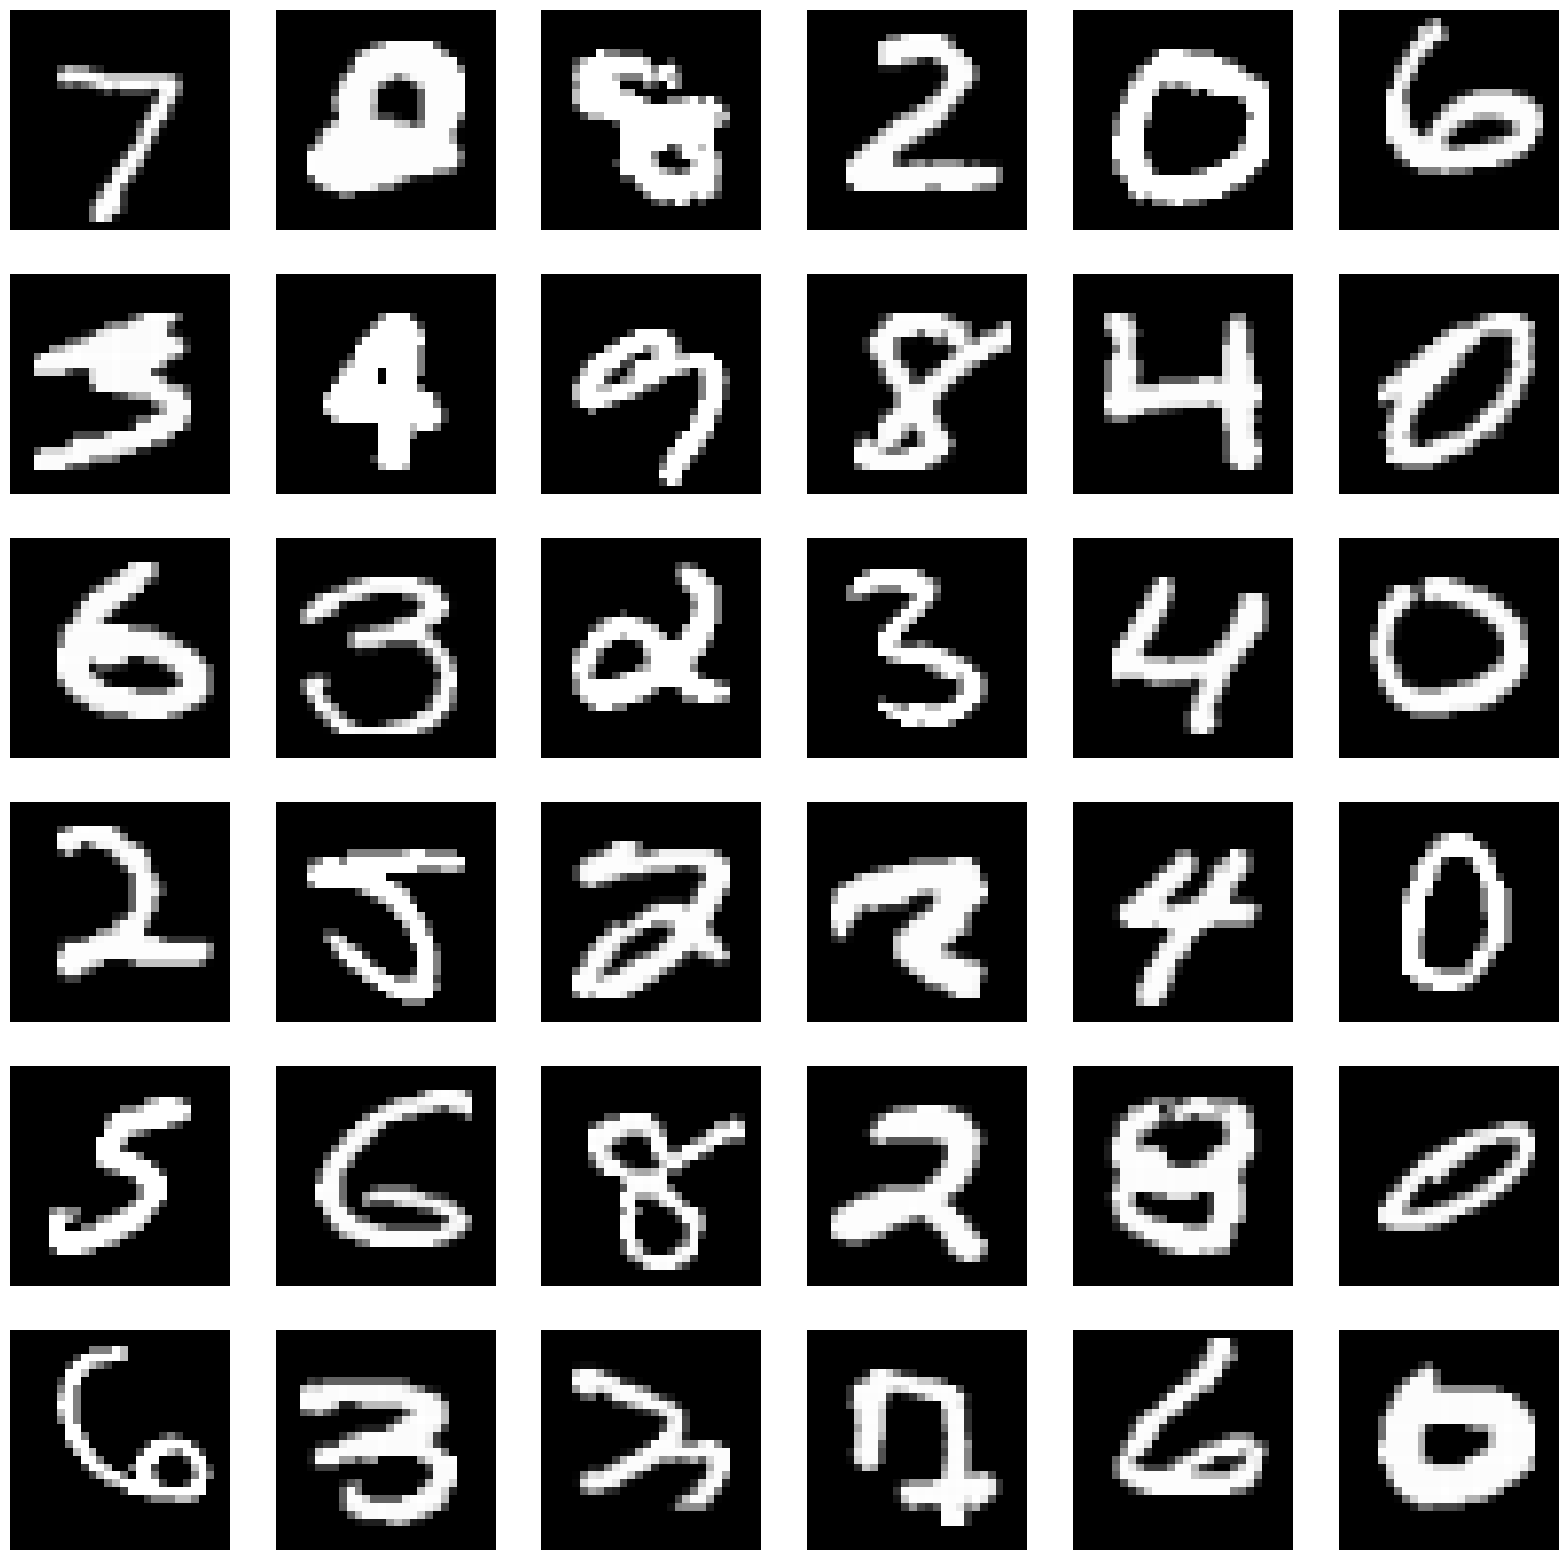
\includegraphics[width=0.65\textwidth]{images/mnist_test_36_0.png}
\end{center}
\caption{mnist Image of k=36 and m=0}
\label{mnist_test_36_0.fig}
\end{figure}


    \item Farthest First Test Task 3 with k = 36 and m = 0
For this farthest first test we will be running the parallel performance of my code.

Figure  
\ref{kmeans_timing_25_0.fig} 
shows our output for a parallel performance when k=36.

\begin{figure}[H]
\begin{center}
    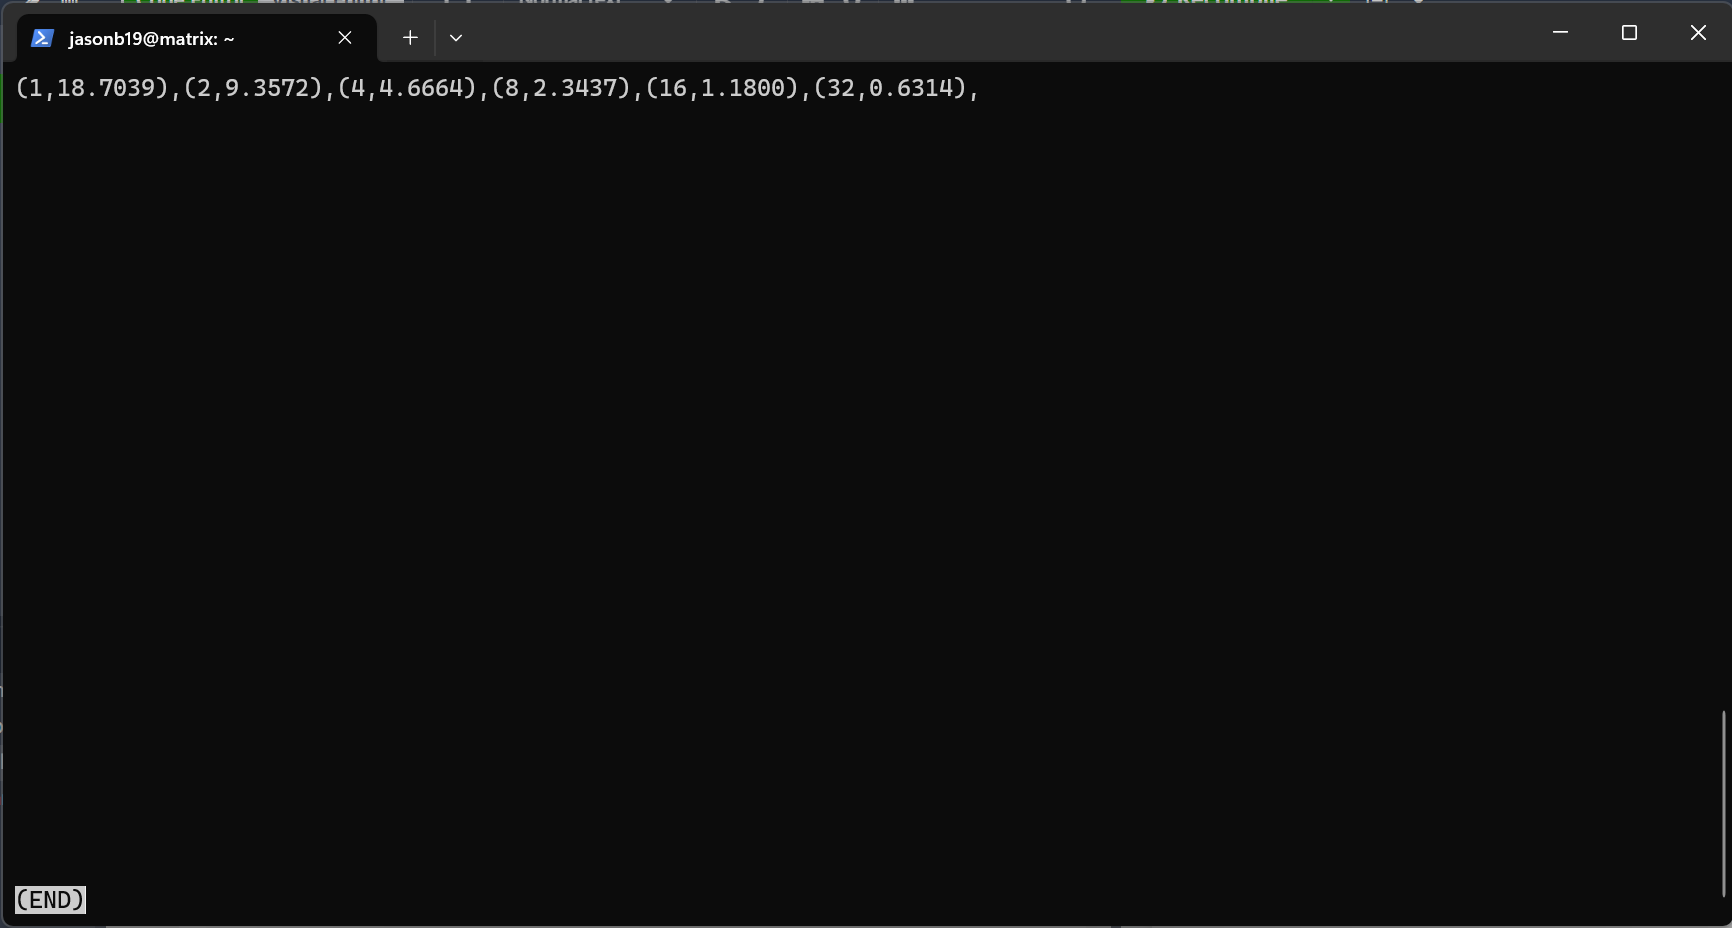
\includegraphics[width=0.95\textwidth]{images/kmeans_timing_36_0.png}
\end{center}
\caption{Parallel Performance for k=36 and m=0}
\label{kmeans_timing_36_0.fig}
\end{figure}

The corresponding strong scaling study of my output is produced:
\begin{verbatim}
[jasonb19@tinkercliffs2 PSA02]$ more omp_kmeans_timing.out
(1,18.7039),(2,9.3572),(4,4.6664),(8,2.3437),(16,1.1800),(32,0.6314),
\end{verbatim}

    \item Scaling Study Plot Generation Figure

Figure  
\ref{plot_36_0.fig} 
is my produced plot for a strong scaling study. This study was conducted using k=36 and m=0.

\begin{figure}[H]
\begin{center}
    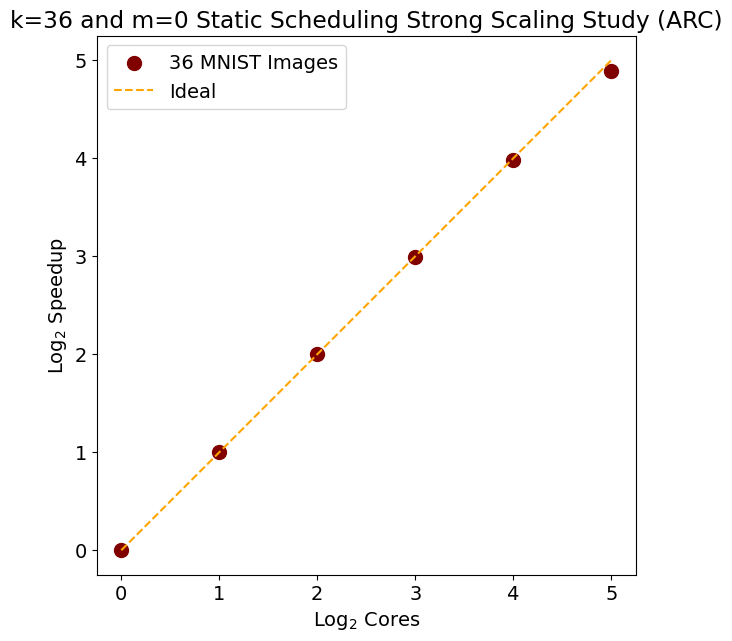
\includegraphics[width=0.95\textwidth]{images/plot_36_0.png}
\end{center}
\caption{Strong Scaling Study for k=36 and m=0 OpenMP}
\label{plot_36_0.fig}
\end{figure}

    
\end{enumerate}

% end of section 3

\section{$k$-means Conceptual and Demonstration Tasks} 

\begin{enumerate}
    \item Classification of Each Variable

% cluster_size(write), k(read), dim(read), num_points(read), kmeans(read), data(read), kmeans_next(read,write)

When evaluating my parallel code, I would review my entire code to see where I can reference my shared variables and private ones. Further examining my code I found that there is only one write variable used, cluster\_size. It is used in my omp critical at the very end. We have plenty of read only variables and only one that is both read-write. kmeans\_next is the only read-write variable. It is used in the function call $vec\_add()$. This function takes in four parameters, the first two being arrays, the third another array, and finally the size of all three arrays. We put the pointer of kmeans\_next into this as the first parameter and our third. Hence, it is reading it and then adding the respective positions of kmeans\_next and our thread\_kmeans\_next and then placing it back into our kmeans\_next. This, along with our cluster\_size are both used to change our values in our omp critical since we want to add up all of our parallel computing at once at the end of our run. Finally, I do believe the remainder of my shared variables are all read only, that being; k, dim, num\_points, kmeans, and data.


    \item Steps Took to Make Code Run Efficiently in Parallel

I began by creating a private variable to be used within our parallel region. This is the values of thread\_cluster\_size with size k, and a thread\_kmeans\_next with size k*dim that. Both are instantiated using all zeros. The first is ran through a for-loop in code, and the next is ran using a function that then runs a similar for-loop. Finally, since most of code is the same, we did not need to change much. A lot of it is read only variables but had to change values of or end result (those that are being changed) with our thread created variables. Such as changing our thread\_cluster\_size within our first for-loop. Finally, in our critical omp we just had to add all of our thread\_cluster\_size evaluations to our cluster\_size, respectively. Finally, we did the same thing by adding our thread\_kmeans\_next variable to our kmeans\_next variable within this same scope (critical omp).


    \item Explanation of Determining Type of Scheduling
    
For Lloyd's algorithm, I incorporated our IF-ELSE condition for if we run DYNAMIC or for our code to run static when prompted. This section comes right before our for-loop and right after instantiating our private thread variables. code:
\begin{verbatim}
 #ifdef DYNAMIC
#pragma omp for schedule(dynamic)
#else
#pragma omp for schedule(static)
#endif
\end{verbatim}
As such, we officially ran our code as static since in compilation I do not believe we called DYNAMIC. I believe we ran static scheduling because our code needed to run in a sequence to find the maximum distance and the minimum cost of the data but for the following set of clusters. I would have to evaluate the one point with another, and then move one to do the same with the next and so one effectively needing to be ordered in a certain way.

    \item Farthest First Test Task 2 with k = 25 and m = 55

We will repeat the farthest first testing task with the new provided values for k and m. Hence, this will be 25 and 55 respectively.

Figure  
\ref{mnist_test_25_55.fig} 
shows our image of the 25 MNIST centers.

\begin{figure}[H]
\begin{center}
    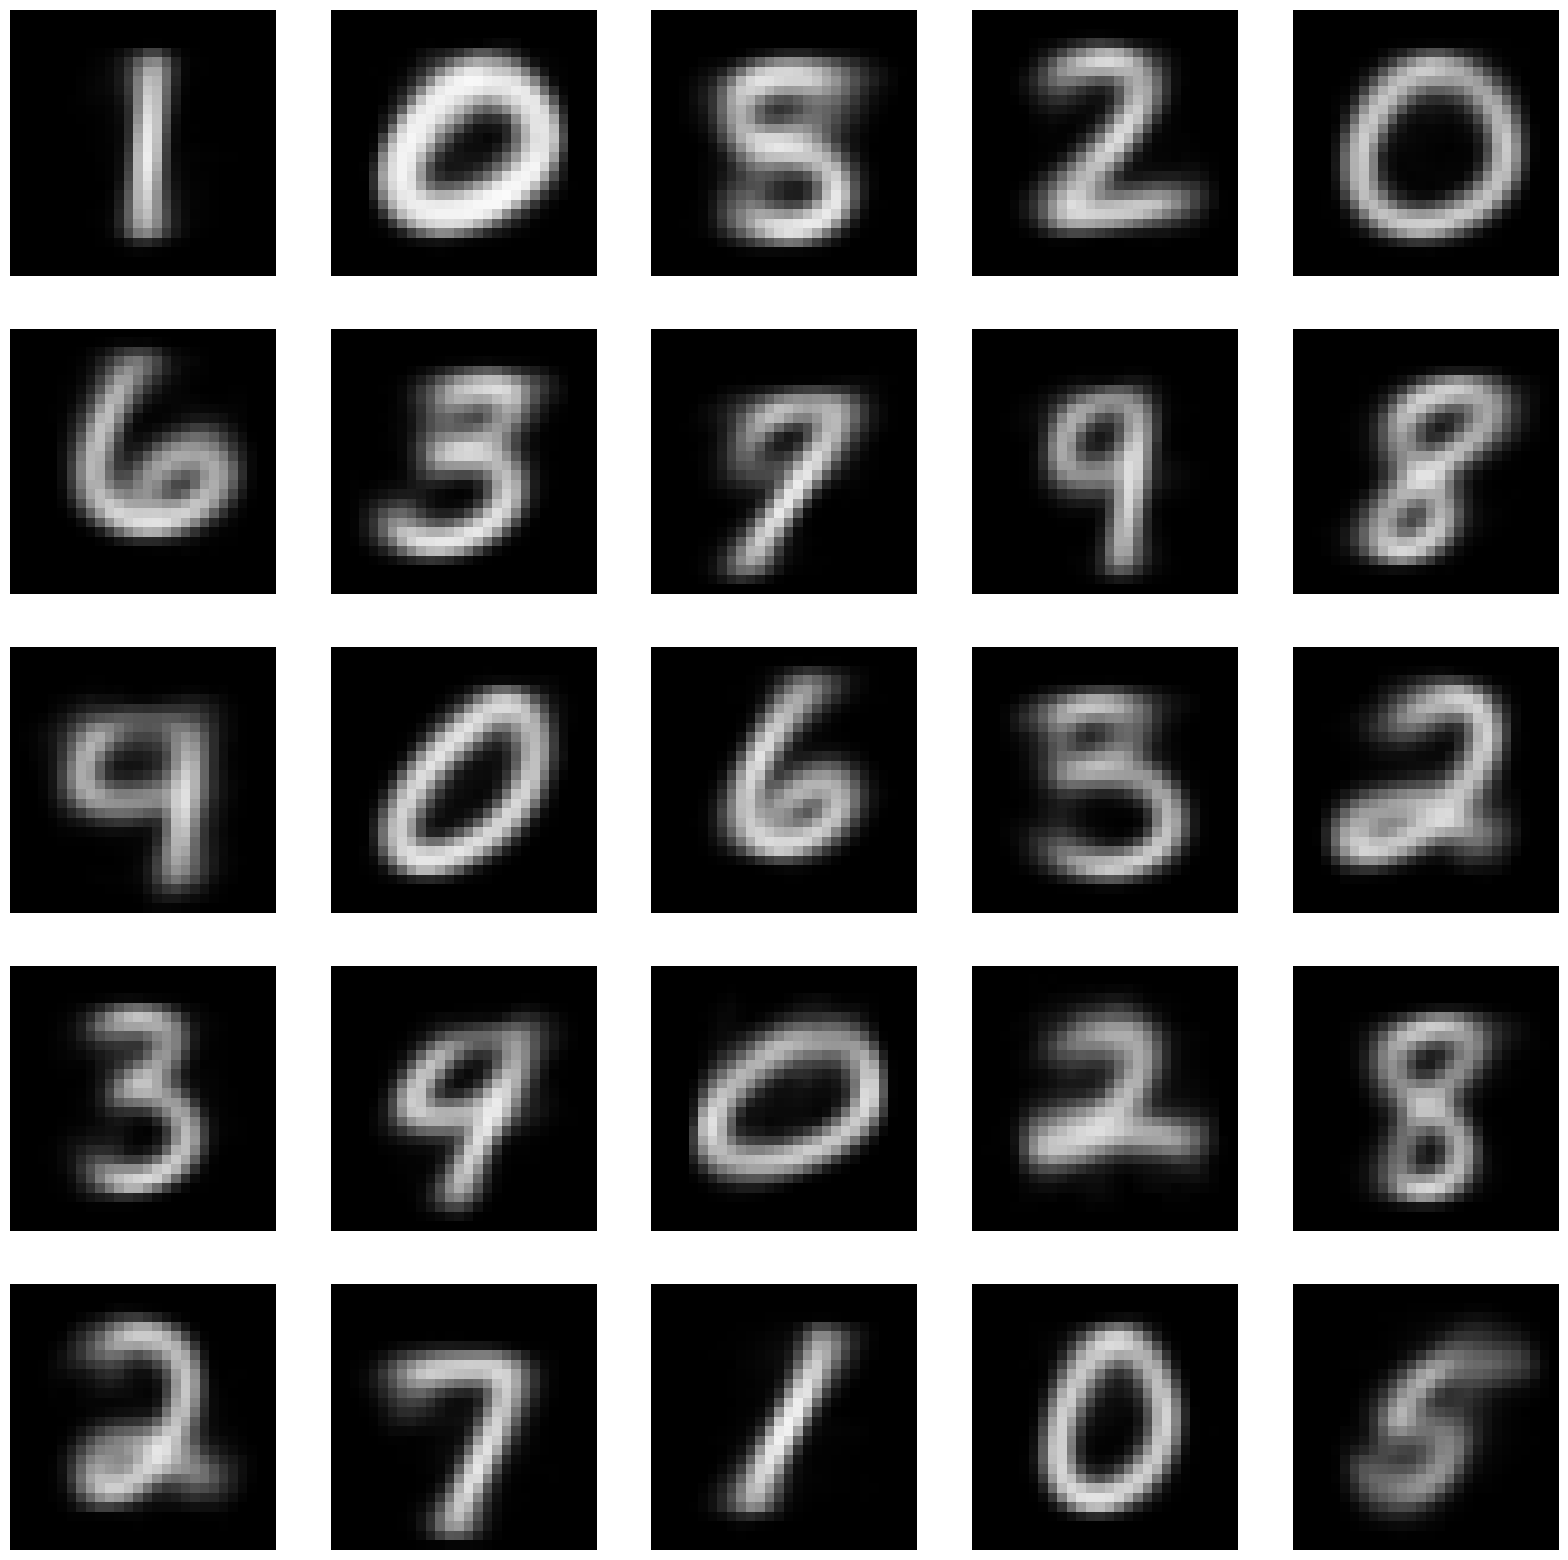
\includegraphics[width=0.65\textwidth]{images/mnist_test_25_55.png}
\end{center}
\caption{mnist Image of k=25 and m=55}
\label{mnist_test_25_55.fig}
\end{figure}

    \item Farthest First Test Task 3 with k = 25 and m = 55
    
For this farthest first test we will be running the parallel performance of my code.

Figure  
\ref{kmeans_timing_25_55.fig} 
shows our output for a parallel performance when k=25.

\begin{figure}[H]
\begin{center}
    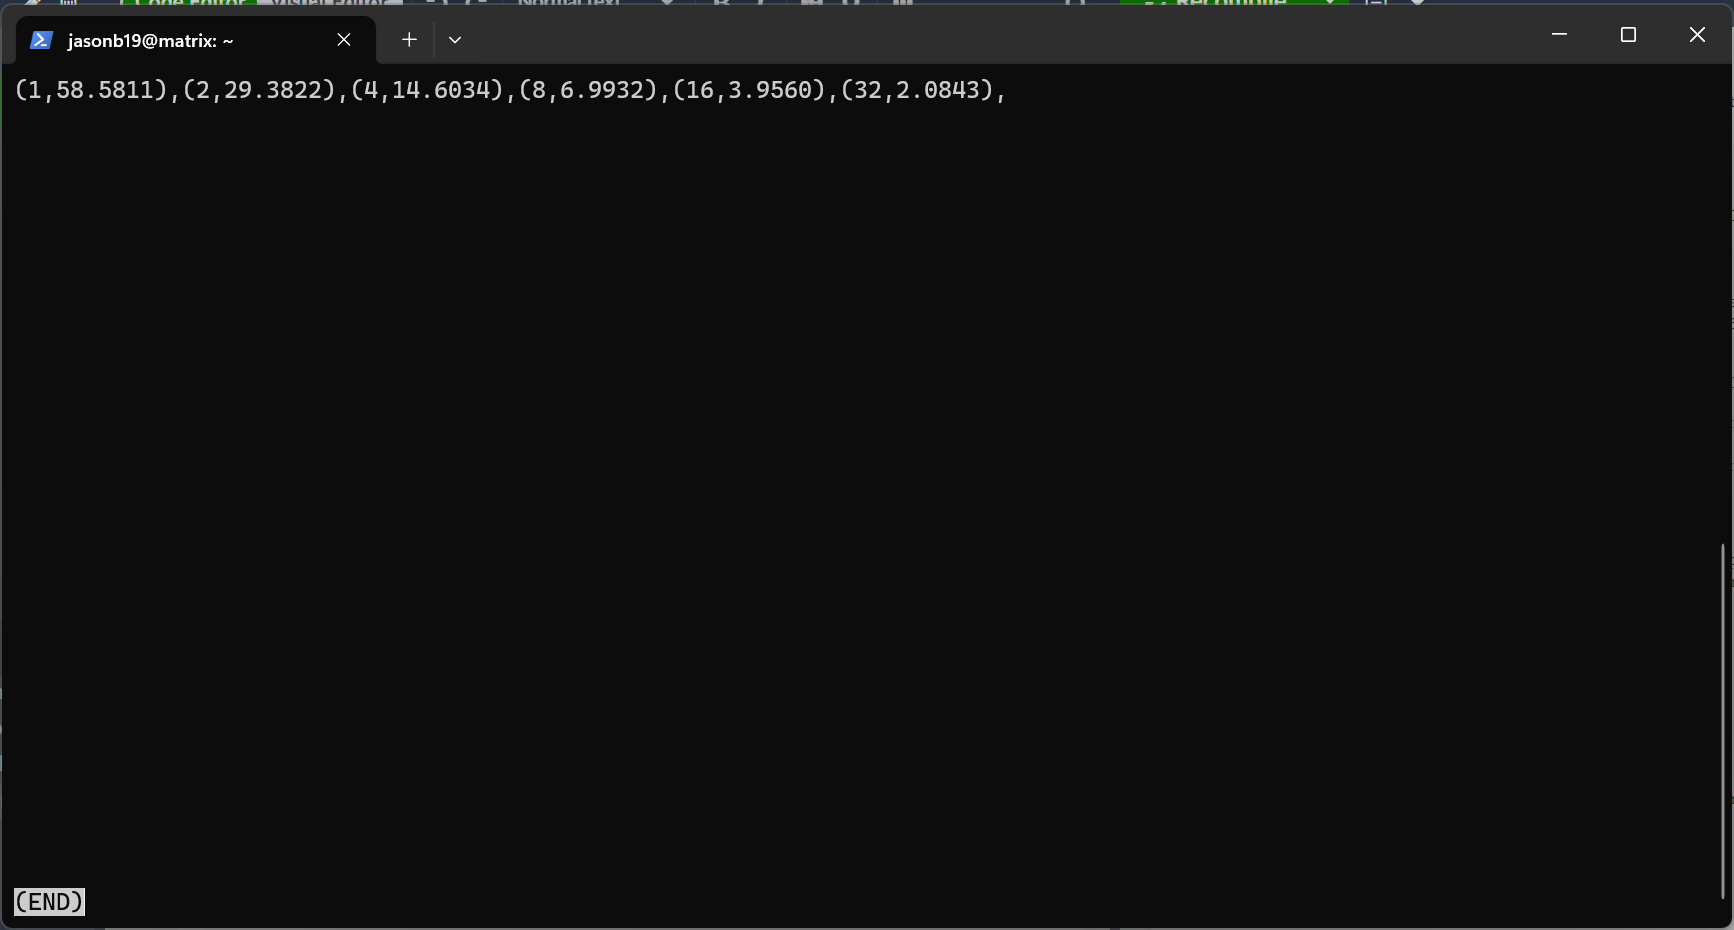
\includegraphics[width=0.95\textwidth]{images/kmeans_timing_25_55.png}
\end{center}
\caption{Parallel Performance for k=25 and m=55}
\label{kmeans_timing_25_55.fig}
\end{figure}


The corresponding strong scaling study of my output is produced:
\begin{verbatim}
[jasonb19@tinkercliffs2 PSA02]$ more omp_kmeans_timing.out
(1,58.5811),(2,29.3822),(4,14.6034),(8,6.9932),(16,3.9560),(32,2.0843),
\end{verbatim}
    \item Scaling Study Plot Generation Figure

Figure  
\ref{plot_25_55.fig} 
is my produced plot for a strong scaling study. This study was conducted using k=25 and m=55.

\begin{figure}[H]
\begin{center}
    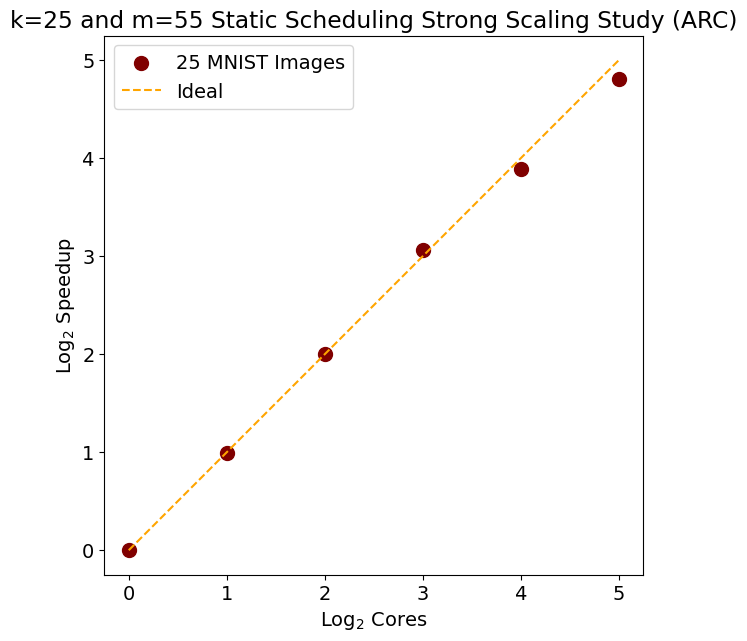
\includegraphics[width=0.95\textwidth]{images/plot_25_55.png}
\end{center}
\caption{Strong Scaling Study for k=36 and m=55 OpenMP}
\label{plot_25_55.fig}
\end{figure}
    
\end{enumerate}



% end of section 4
\end{document}
